
相关阅读: 双联通分量 

\subsection{割点}

\begin{QUOTE}{}{}
如果在一个图中,如果把一个点删除,那么这个图不再联通,那么这个点就是割点(割顶),当然是在无向图。
\end{QUOTE}

\subsubsection{如何实现?}

如果我们尝试删除每个点,并且判断这个图的联通性,那么复杂度会特别的高。所以要介绍一个常用的算法:$Tarjan$。

首先,我们上一个图:

\begin{figure}[htbp]
\centering
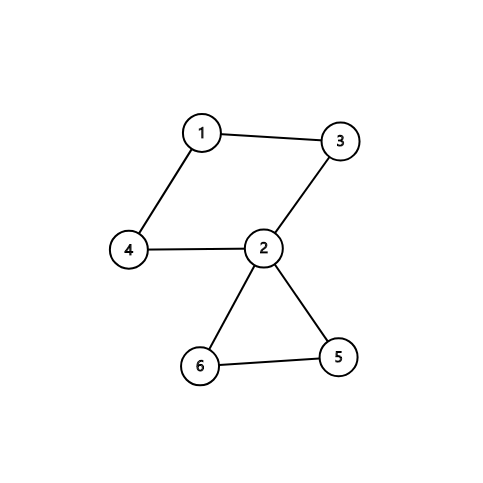
\includegraphics[width=0.7\textwidth]{docs/graph/images/bridge1.png} 

\end{figure}

很容易的看出割点是 2,而且这个图仅有这一个割点。

首先,我们按照 $DFS$ 序给他打上时间戳(访问的顺序)。

\begin{figure}[htbp]
\centering
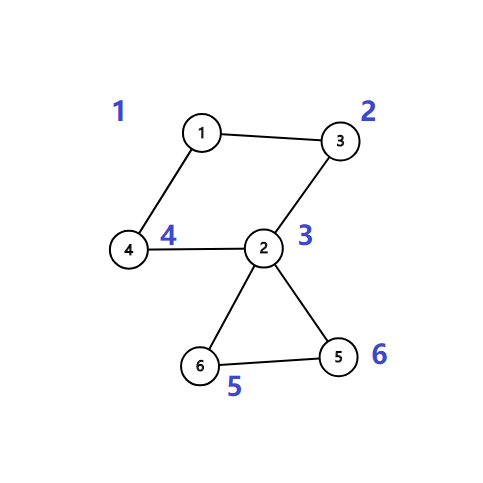
\includegraphics[width=0.7\textwidth]{docs/graph/images/bridge2.png} 

\end{figure}

这些信息被我们保存在一个叫做 \texttt{num} 的数组中。

还需要另外一个数组 \texttt{low},用它来存储不经过其父亲(你有多个那么就看你遍历到了哪个)能到达的时间戳。

例如 2 的话是 1, 5 和 6 是 3。

然后我们开始 $DFS$,我们判断某个点是否是割点的根据是:对于某个顶点 $u$,如果存在至少一个顶点 $v$ ( $u$ 的儿子),使得 $low_v>=num_u$,即不能回到祖先,那么 $u$ 点为割点。

另外,如果搜到了自己(在环中),如果他有两个及以上的儿子,那么他一定是割点了,如果只有一个儿子,那么把它删掉,不会有任何的影响。比如下面这个图,此处形成了一个环,从树上来讲它有 2 个儿子:

\begin{figure}[htbp]
\centering
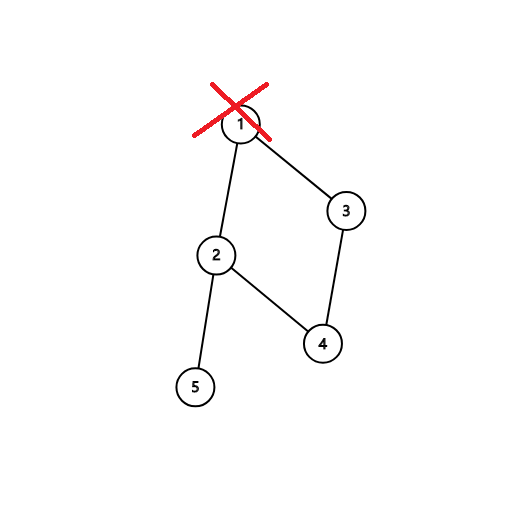
\includegraphics[width=0.7\textwidth]{docs/graph/images/bridge3.png} 

\end{figure} 

我们在访问 1 的儿子时候,假设先 $DFS$ 到了 2,然后标记用过,然后递归往下,来到了 4, 4 又来到了 3,当递归回溯的时候,会发现 3 已经被访问过了,所以不是割点。

更新 \texttt{low} 的伪代码如下:

\begin{cppcode}
如果 v 是 u 的儿子 low[u] = min(low[u], low[v]);
否则
low[u] = min(low[u], num[v]);
\end{cppcode}

\subsubsection{例题}

\href{https://www.luogu.org/problemnew/show/P3388}{洛谷 P3388 【模板】割点(割顶)}

\subsubsection{Code}

\begin{cppcode}
/*
洛谷 P3388 【模板】割点(割顶)
*/
#include <bits/stdc++.h>
using namespace std;
int n, m;  // n:点数 m:边数
int num[100001], low[100001], inde, res;
// num:记录每个点的时间戳
// low:能不经过父亲到达最小的编号,inde:时间戳,res:答案数量
bool vis[100001], flag[100001];  // flag: 答案 vis:标记是否重复
vector<int> edge[100001];        // 存图用的
void Tarjan(int u, int father)  // u 当前点的编号,father 自己爸爸的编号
{
  vis[u] = true;             // 标记
  low[u] = num[u] = ++inde;  // 打上时间戳
  int child = 0;             // 每一个点儿子数量
  for (auto v : edge[u])     // 访问这个点的所有邻居 (C++11)
  {
    if (!vis[v]) {
      child++;                       // 多了一个儿子
      Tarjan(v, u);                  // 继续
      low[u] = min(low[u], low[v]);  // 更新能到的最小节点编号
      if (father != u && low[v] >= num[u] &&
          !flag
              [u])  // 主要代码
                    // 如果不是自己,且不通过父亲返回的最小点符合割点的要求,并且没有被标记过
                    // 要求即为:删了父亲连不上去了,即为最多连到父亲
      {
        flag[u] = true;
        res++;  // 记录答案
      }
    } else if (v != father)
      low[u] =
          min(low[u], num[v]);  // 如果这个点不是自己,更新能到的最小节点编号
  }
  if (father == u && child >= 2 &&
      !flag[u])  // 主要代码,自己的话需要 2 个儿子才可以
  {
    flag[u] = true;
    res++;  // 记录答案
  }
}
int main() {
  cin >> n >> m;                // 读入数据
  for (int i = 1; i <= m; i++)  // 注意点是从 1 开始的
  {
    int x, y;
    cin >> x >> y;
    edge[x].push_back(y);
    edge[y].push_back(x);
  }                             // 使用 vector 存图
  for (int i = 1; i <= n; i++)  // 因为 Tarjan 图不一定联通
    if (!vis[i]) {
      inde = 0;      // 时间戳初始为 0
      Tarjan(i, i);  // 从第 i 个点开始,父亲为自己
    }
  cout << res << endl;
  for (int i = 1; i <= n; i++)
    if (flag[i]) cout << i << " ";  // 输出结果
  for (int i = 1; i <= n; i++) cout << low[i] << endl;
  return 0;
}
\end{cppcode}

\subsection{割边}

和割点差不多,还叫做割桥。

\begin{QUOTE}{}{}
无向联通图中,去掉一条边,图中的连通分量数增加,则这条边,称为桥或者割边,当然也是在无向图。
\end{QUOTE}

\subsubsection{实现}

和割点差不多,只要改一处: $low_v>num_u$ 就可以了,而且不需要考虑根节点的问题。

割边是和是不是根节点没关系的,原来我们求割点的时候是指点 $v$ 是不可能不经过父节点 $u$ 为回到祖先节点(包括父节点),所以顶点 $u$ 是割点。如果 $low_v==num_u$ 表示还可以回到父节点,如果顶点 $v$ 不能回到祖先也没有另外一条回到父亲的路,那么 $u-v$ 这条边就是割边

$Tarjan$ 算法还有许多用途,常用的例如求强连通分量,缩点,还有求 $2-SAT$ 的用途等。
